\section{Análisis}
En esta sección se realizará una planificación temporal detallada del proyecto, teniendo en cuenta las actividades necesarias para su desarrollo y los plazos asociados.

    \subsection{Análisis de Requisitos}
        \subsubsection{Requisitos Funcionales}
            \begin{enumerate}
                \item \textbf{Generación de terreno infinito:} El sistema debe ser capaz de generar chunks ilimitados de terreno de manera procedural en tiempo real, permitiendo a los usuarios especificar los parámetros como altura del terreno, escala de frecuencia, nivel del mar, etc.
                \item \textbf{Generación de biomas:} El terreno generado debe tener regiones diferenciadas que representen distintos ecosistemas.
                \item \textbf{Personalización de biomas:} Permitir al usuario personalizar los biomas generados, como la distribución de la vegetación, tipos de vegetación, texturas, etc.
                \item \textbf{Generación de poblaciones:} Sobre el terreno deberán aparecer poblaciones en base a las características del terreno, siendo  estas mayores o menores según las características del terreno donde se generen.
                \item \textbf{Parametrización de las generaciones:} Tanto el terreno, como los biomas y poblaciones deben ser controlables por el usuario mediante parámetros en mayor o menor grado.
                \item \textbf{Distribución de elementos:} A la hora de generar biomas se deben distribuir elementos ambientales como vegetación, rocas u otros objetos ambientales.
                \item \textbf{Detección de colisiones:} El sistema deberá implementar colisiones para que el usuario pueda moverse sobre la superficie del terreno sin atravesar el suelo o las pendientes gracias al sistema de físicas de Unity y su detección de colisiones.
                \item \textbf{Texturización:} El terreno debe ser texturizado con el mezclado de varias texturas. 
                \item \textbf{Texturas configurables:} Al igual que los algoritmos de generación, las texturas también han de poder ser configuradas por el usuario, permitiendo establecer qué aspecto se quiere en cada nivel de altura del terreno.
                \item \textbf{Optimización mediante DOTS: }El sistema debe estar optimizado usando el sistema DOTS de Unity.
                \item \textbf{Técnicas de optimización: } Además del sistema DOTS, se deben implementar otras técnicas de optimización como culling y LOD.
                \item \textbf{Sistema de sonido: }El sistema debe añadir sonidos adaptados al entorno donde se encuentre el usuario.
                \item \textbf{Exportación de terreno:} Proporcionar la capacidad de exportar el terreno generado en un formato compatible con otros programas o motores de juego.
                \item \textbf{Integración de assets externos:} Permitir la integración de assets externos, como modelos 3D de edificios, plantas o rocas, texturas o sonidos.
            
            \end{enumerate}
        \subsubsection{Requisitos No Funcionales}
            \begin{enumerate}
                \item \textbf{Continuidad del terreno:} El terreno no debe presentar discontinuidades y debe generar chunks de terreno sin que haya una transición notable de uno a otro.
                \item \textbf{Distribución de elementos no uniforme:} En la naturaleza es raro que las plantas y otros elementos del paisaje se distribuyan de manera uniforme, por lo que se evitará esta distribución.
                \item \textbf{Realismo visual:} El terreno generado debe ser realista, incluyendo detalles naturales y accidentes geológicos.
                \item \textbf{Usabilidad:} El sistema debe ser intuitivo, con parámetros nombrados de manera que no causen confusión en el usuario y expresen de manera clara su función.
                \item \textbf{Rendimiento:} Se debe ser capaz de generar terrenos en tiempo real con una buena tasa de refresco.
                \item \textbf{Compatibilidad con RV:} El sistema debe permitir generar terrenos en RV proporcionando una buena experience inmersiva.
                \item \textbf{Control de mareos:} El sistema no debe propiciar la aparición de mareos debido a su mal funcionamiento cuando se use en RV.
                \item \textbf{Control de vértices y polígonos:} Los assets que se integren deberán cumplir ciertas condiciones para que no entorpezcan el rendimiento mínimo del sistema.
                \item \textbf{Escala del terreno y elementos:} La generación debe ser a escala 1:1 para dar una sensación de inmersividad real.
                \item \textbf{Intensidad baja del sonido:} Dado que el sonido tendrá fin ambiental, un sonido de alta intensidad distorsionaría la experiencia.
            \end{enumerate}

    \subsection{Análisis Temporal}
        \subsubsection{Desglose de Tareas}
        \begin{enumerate}
            \item \textbf{Estudio preliminar:} Esta tarea consiste en hacer una recopilación de los requisitos y objetivos a cumplir, así como la planificación y estudio de la viabilidad del proyecto del estado del arte referente a este proyecto.
            \item \textbf{Análisis:} En el análisis se analizarán los requisitos que se exigirán a este proyecto, se estudiarán los componentes y partes del sistema que se implementará, así como la integración que estos tendrán y se analizarán los comportamientos y resultados que se deben producir durante su funcionamiento.
            \item \textbf{Diseño:} Esta tarea se centra en cómo se va a construir el sistema esclareciendo los componentes y definiendo especificaciones usando para ello diferentes diagramas.
            \item \textbf{Implementación:} La tarea que consiste en la programación de la propia propuesta y la realización de las pruebas pertinentes, así como sus posibles mejoras y extensiones.
            \item \textbf{Resultados y conclusiones:} En esta tarea se hará una revisión de la solución desarrollada y sus resultados, analizando las diferentes pruebas que muestran cuáles son sus capacidades, obteniendo conclusiones sobre su desempeño y estableciendo posibles líneas de trabajo futuro.
            \item \textbf{Documentación:} La documentación es la tarea que recoge las actividades de elaboración de la memoria, la presentación y de video demostrativo, que documenta el proceso de elaboración del proyecto y su funcionamiento.
        \end{enumerate}
        
        \subsubsection{Estimación de Tiempos}
        Para el cálculo temporal de cada tarea se realizará un cálculo estimado basado en la siguiente fórmula:
        \begin{equation}
            te = to + \frac{4tm + tp}{6} \label{eq:temporal}
        \end{equation}
        Donde $te$ es el tiempo estimado, $to$ el tiempo optimista, $tp$ es el tiempo pesimista y $tm$ es el tiempo probable.

        Una vez determinados los tiempos estimados del total del proyecto por los expertos, se hará un cálculo ponderado del mismo en base a unos pesos que tendrá cada estimación según la fórmula:
        \begin{equation}
            te = exp1 \times 0.5 + exp2 \times 0.35 + exp3 \times 0.15 \label{eq:ponderado}
        \end{equation}
        Donde $exp1$ es el tiempo estimado calculado con la fórmula \ref{eq:temporal} del experto 1, $exp2$ el tiempo estimado del experto 2 y $exp3$ el tiempo estimado del experto 3.

        Los expertos y sus pesos en el cálculo final del tiempo estimado son los siguientes \footnote{Todos los tiempos serán medidos en días}:
        \begin{itemize}
            \item 
        \end{itemize}

        \begin{figure}
            \centering
            \includegraphics[width=1\textwidth]{img/estimación-temporal.png}
            \caption{Estimación de ..., primer experto.}
            \label{fig:estimacion1}
        \end{figure}

        \begin{figure}
            \centering
            \includegraphics[width=1\textwidth]{img/estimación-temporal.png}
            \caption{Estimación de ..., segundo experto.}
            \label{fig:estimacion2}
        \end{figure}

        \begin{figure}
            \centering
            \includegraphics[width=1\textwidth]{img/estimación-temporal.png}
            \caption{Estimación de ..., tercer experto.}
            \label{fig:estimacion3}
        \end{figure}

        Una vez calculados los tiempos estimados por los expertos hay que aplicar los pesos para calcular las ponderaciones. El tiempo estimado ponderado queda tal que:

        \begin{figure}
            \centering
            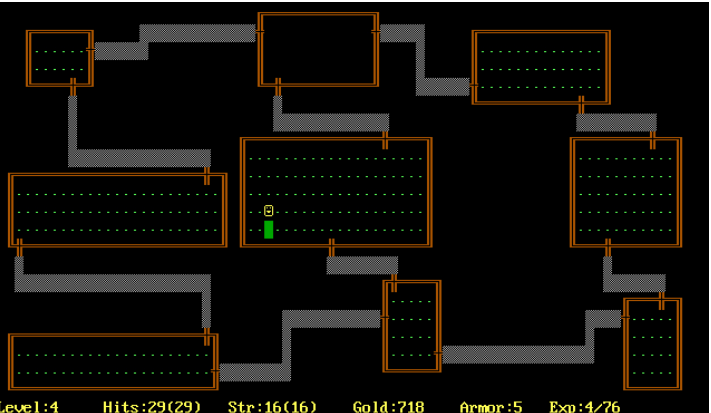
\includegraphics[width=0.5\textwidth]{img/Rogue.png}
            \caption{Tiempos estimados ponderados.}
            \label{fig:tiempos-ponderados}
        \end{figure}
        
        Además de los tiempos ponderados también se ha decidido calcular otros datos de interés como son la desviación típica $\sigma^2$ y la varianza $\sigma$ para determinar la desviación de los valores respecto del promedio.

        \begin{equation}
            \sigma^2 = \left(\frac{tp - to}{6}\right)^2 \label{eq:varianza}
        \end{equation}
        
        \begin{equation}
            \sigma = \sqrt{\sigma^2} \label{eq:desviacion}
        \end{equation}
        
        % \begin{figure}[h]
        %     \centering
        %     \includegraphics[width=0.5\textwidth]{img/varianzas-y-desviaciones.png}
        %     \caption{Varianzas y desviaciones típicas respecto a los valores promedios.}
        %     \label{fig:varianzas-desviaciones}
        % \end{figure}
        
        Gracias a estos valores podemos hacer un cálculo de cuál podría ser el tiempo de realización del proyecto en base a las estimaciones de los expertos con determinados niveles de confianza. Calcularemos el tiempo que se tardaría en realizar el proyecto según la estimación de los expertos con un 90\% de confianza y con un 99\% de confianza usando la distribución normal estándar para cálculo de probabilidades de variables aleatorias continuas. La fórmula para el cálculo de probabilidad es la siguiente:
        
        \begin{equation}
            Z = \frac{X - \mu}{\sigma} \label{eq:probabilidad}
        \end{equation}
        
        Con un 90\% de confianza, mirando en la tabla el valor de Z es 1,2815:
        
        \[
        1,2815 = \frac{X - 154,20}{57,83}; \quad X = 228,3
        \]
        
        Con un 99\% de confianza, mirando en la tabla el valor de Z es 2,3263:
        
        \[
        2,3263 = \frac{X - 154,20}{57,83}; \quad X = 288,73
        \]
        
        Según los cálculos, con un 90\% de confianza, el proyecto debería terminarse en  días y con un porcentaje del 99\%, el proyecto debería terminarse en 288 días como máximo.
        

        \subsubsection{Diagrama de Gantt}
        Para visualizar la estimación temporal que se ha hecho de las tareas se ha realizado un diagrama de Gantt. El diagrama se puede ver en la \hyperref[fig:gantt]{imagen del anexo}.


    \subsection{Análisis Económico}

        \subsubsection{Costes Directos}
            \paragraph{Costes de hardware}
            En este apartado se calculará el costo del equipo necesario para desarrollar este proyecto, así como su amortización. El material requerido para este proyecto incluye un ordenador portátil con las \hyperref[subsec:Especificación del Equipo]{especificaciones} definidas en el apéndice, así como un ratón, ya que es necesario para navegar por el entorno 3D de la interfaz de Unity.

            El costo de la computadora portátil es de 1000 euros aproximadamente, con una amortización máxima de 5 años según la Agencia Tributaria \cite{agencia_tributaria_tabla_2024}, el del ratón es de 15 euros y las gafas de RV 500 euros, con un tiempo máximo de amortización de 5 años ambos también al tratarse de útiles, herramientas o equipos para el tratamiento de la información y sistemas informáticos. De los tres componentes del equipo se han utilizado al 100 \% durante el proyecto el ordenador portátil y el ratón, mientras que las gafas se han usado en las pruebas y mejoras hechas de la fase de pruebas para la compatibilidad con RV, por lo que se estima que se han usado entorno a un 20\% y un 10\% del total del proyecto, considerando la media: 15\% como su \% de uso aproximado final. Con estos datos, el costo amortizado se calcula de la siguiente manera:

            \[ \text{Coste amortizado} = \text{Días de uso} \times \text{\% de uso} \times \text{Precio de amortización por día} \]

            Donde el precio de amortización por día se calcula como:

            \[ \text{Precio de amortización por día} = \frac{\text{precio}}{\text{vida útil}} \]

            Dado que el tiempo de vida útil de un ordenador portátil se estima en aproximadamente 5 años y el de un ratón en 3 años, mientras que el de las gafas de RV no tienen una estimación estima entre 2 y 5 años, por lo que las estimaremos en 3,5 años. Por lo tanto, el cálculo del precio de amortización se realiza de la siguiente manera:

            \begin{figure}[H]
                \centering
                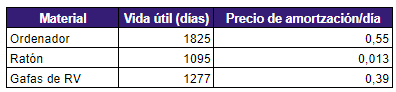
\includegraphics[width=0.65\textwidth]{img/precio-amortizado.png}
                \caption{Amortización por día.}
                \label{fig:amortización-diaria}
            \end{figure}

            Por tanto las amortizaciones del equipo queda así:

            \begin{figure}[H]
                \centering
                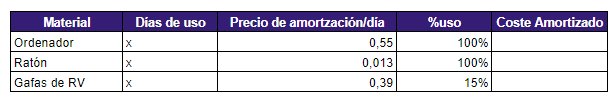
\includegraphics[width=0.85\textwidth]{img/coste-amortizado.png}
                \caption{Costes amortizados del equipo.}
                \label{fig:coste-amortizado}
            \end{figure}

            El ordenador tiene una amortización de x/€ por día y el ratón de y/€ por día. Lo
            que supone un total de z/€ amortizados por día.


            \paragraph{Costes de software}
            Son los costes asociados a los programas necesarios para el desarrollo del proyecto.
            En este caso, todos los recursos software utilizados han sido gratuitos, ya que Unity es
            un software gratuito, se ha usado VS Code como editor de código, el cual también es gratuito, así como Git y Trello.
            Los softwares con los que se ha gestionado el proyecto para creación de diagramas han sido softwares online gratuitos y para las presentaciones se han utilizado los documentos que ofrece Google. Los costes en software por lo tanto han sido 0.

        \subsubsection{Costes Indirectos}
        En cuanto a los costes indirectos, se necesitaría al menos de un lugar de trabajo, luz, agua e internet que suponen unos gastos mensuales adicionales:
        \begin{figure}[H]
            \centering
            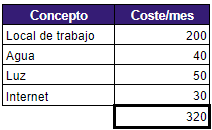
\includegraphics[width=0.35\textwidth]{img/costes-indirectos.png}
            \caption{Costes indirectos.}
            \label{fig:costes-indirectos}
        \end{figure}

        Dado que el tiempo necesitado en este proyecto ha sido de X días, lo que equivale a no se cuantos meses, por tanto:
        \[ \text{meses que dura el proyecto} \times \frac{\text{costes indirectos}}{\text{mes}} = \text{costes indirectos totales} \]

        Finalmente, los costes totales del proyecto quedan tal que:

        \begin{figure}[H]
            \centering
            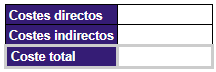
\includegraphics[width=0.35\textwidth]{img/costes-totales.png}
            \caption{Costes totales del proyecto.}
            \label{fig:costes-indirectos}
        \end{figure}

        En resumen, el proyecto ha tenido una duración de X días, Y horas y un coste total de Z €. 
        
        El coste temporal del proyecto es debido en su gran parte al trabajo de investigación previo realizado, pues el tema de este proyecto ha sido estudiado desde hace décadas generando gran cantidad de artículos y material que revisar. También la inexperiencia en el uso de tecnologías como el sistema DOTS de Unity que ha requerido un proceso de aprendizaje para adaptar el código a la estructura de este sistema. Además, las pruebas necesarias para comprobar la correcta integración y funcionamiento de todos los componentes y su adaptación a la realidad virtual, sin ser un desarrollador experto en ella, ha sido otros de los factores claves que justifican el coste temporal del proyecto.

    \subsection{Análisis de Viabilidad}
        \subsubsection{Viabilidad Técnica:}
        \subsubsection{Viabilidad Económica}
        \subsubsection{Viabilidad Legal}
        \subsubsection{Análisis de Riesgos}

    
    \subsection{Diagramas de Análisis}

        \subsubsection{Diagrama de Casos de Uso}
        \subsubsection{Otros Diagramas de Análisis}

    \subsection{Conclusiones del Análisis}

